\newpage
\section{Geometria trifocal}\label{sec.geo-tri}
Assim como num sistema com duas imagens, podemos extrair informações sobre o cenário em 3D através da correspondência entre pontos, retas, tangentes e segmentos de curvas com três  ou mais imagens. No entanto, grande parte das pesquisas em visão computacional não tem utilizado a geometria trifocal em problemas de reconstrução 3D e transferência de pontos de uma imagem para outra. Menor ainda é a utilização da geometria diferencial para abordar esses problemas para curvas gerais, tais como cristas de ondas. Um dos nossos objetivos é fazer um levantamento das características e conceitos encontrados num sistema trifocal em comparação com a geometria epipolar, e relatar alguns dos benefícios conseguidos através da inclusão de uma terceira imagem.

\begin{figure}[htb!]
\centering
\subfloat{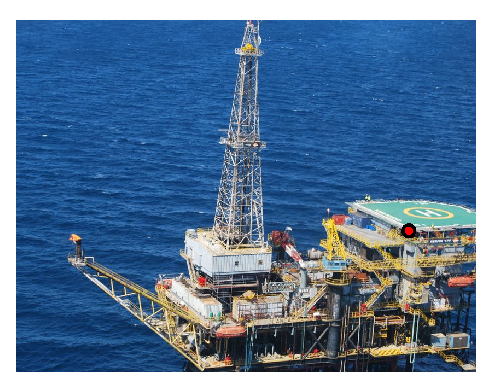
\includegraphics[scale=.67]{plataforma-1}}
\quad
\subfloat{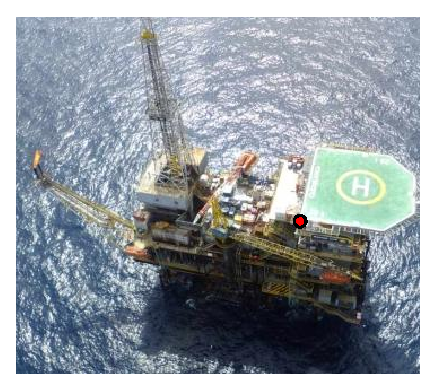
\includegraphics[scale=.67]{plat-2}}
\quad
\subfloat{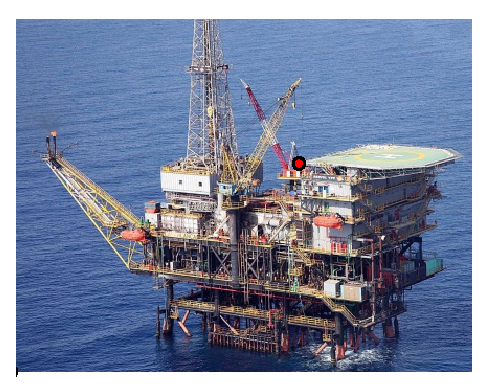
\includegraphics[scale=.67]{plat-3}}
\caption{{\it Três imagens da plataforma petrolífera espanhola Casablanca. Exemplo de três pontos correspondentes em vermelho representando um canto do heliporto.}}
\end{figure}

\subsection{O Problema}
Considere um cenário em 3D com três imagens em 2D desse cenário conforme a figura \ref{fig.trifocal-frente}, onde podemos visualizar as três imagens $\x$, $\x'$ e $\x''$ de um ponto 3D $\X$ (dois sinais de apóstrofo indicam o objeto pertencente à terceira câmera) e os pontos correpondentes $\x\leftrightarrow\x'\leftrightarrow\x''$ são previamente conhecidos. O desafio da reconstrução 3D é determinar, a partir das correspondências nas imagens, as matrizes das câmeras $P$, $P'$ e $P''$ que realizam as projeções $\x=P\,\X$, $\x'=P'\X$ e $\x''=P''\X$ em cada imagem, bem como a determinação do ponto $\X$. Nesse trabalho está sendo dada prioridade à determinação das matrizes das câmeras, por ser um dos maiores problemas atuais em visão computacional e que torna-se primordial no caso de curvas \citep{tese-fabbri}.

É mais comum a utilização da geometria epipolar bifocal para problemas de reconstrução 3D, fazendo a extração das câmeras usando a geometria epipolar e aplicando um algoritmo para determinação do ponto 3D a partir da triangulação $(\x,\x',\X)$. Mas quando aumentamos para três a quantidade de imagens, aumentam-se também as possibilidades de degenerações (que depende  da posição do ponto 3D $\X$) se continuarmos utilizando as ferramentas da geometria epipolar a cada par de imagens. Mostraremos que alguns casos de degenerações podem ser removidos usando a teoria da geometria trifocal.


Vamos aplicar o procedimento contido em \citep{Faugeras} que consiste em utilizar a geometria epipolar bifocal num problema de transferência de pontos num sistema trifocal, avaliar as deficiências dessa abordagem e em seguida mostrar como a geometria trifocal pode erradicar algumas dessas deficiências. 
\begin{figure}
\centering
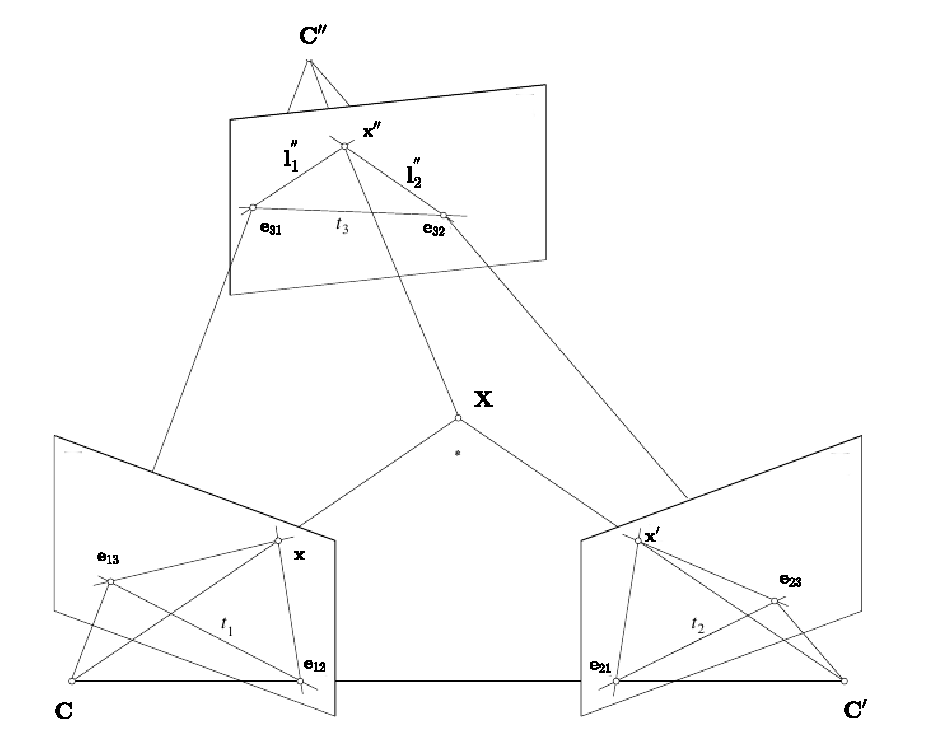
\includegraphics[scale=.8]{trifocal-frente-frente}
\caption{{\it O plano trifocal juntamente com os três planos epipolares. A transferência epipolar falha em alguns casos.}}
\label{fig.trifocal-frente}
\end{figure}

O plano definido pelos pontos $\C, \C' \,\,\text{e}\,\, \X$ forma o plano epipolar para as câmeras 1 e 2. Analogamente, temos o plano epipolar para as câmeras 1 e 3 e para as câmeras 2 e 3. A interseção de cada plano epipolar com os planos das imagens geram as retas epipolares. Por exemplo, a reta  epipolar $\lightrgb''_1$ definida pelos pontos $\e_{31}$ e $\x''$ na terceira imagem, é a reta epipolar com relação ao ponto $\x$ na primeira imagem. Ou seja, $\lightrgb''_1$ é a imagem, na câmera 3, da reta retroprojetada por $\x$ através do centro de projeção $\C$ na câmera 1. Essa reta é definida por $\lightrgb''_1=F_{31}\,\x$ ou $\lightrgb''_1=\e_{31}\times\x''$, onde $F_{ij}$ é a matriz fundamental para as câmeras $i$ e $j$ tomando como base a câmera $j$. O plano formado pelos centros de projeção $\C, \C' \,\,\text{e}\,\, \C''$ é chamado {\it plano trifocal} e as interseções desse plano com os planos das imagens geram as {\it retas trifocais} denotadas por ${\bf t}_i$.

\subsection{Transferência epipolar}\label{sec.trans-epipolar}
Supondo que temos os pontos correspondentes $\x\leftrightarrow\x'$ para as câmeras 1 e 2, bem como as matrizes fundamentais para os três planos epipolares da figura \ref{fig.trifocal-frente}, $F_{21}$, $F_{31}$ e $F_{32}$, desejamos determinar as coordenadas do ponto $\x''$ no plano de imagem da câmera 3. Como vimos, os pontos $\x$, $\x'$ e $\x''$ são imagens de um mesmo ponto 3D $\X$, e por isso $\x''$ é um ponto correspondente ao ponto $\x$ e, portanto, $\x''\in\lightrgb''_1$, onde $\lightrgb''_1=F_{31}\x$ é a reta epipolar para as câmeras 1 e 3. Por um argumento similar, constatamos que $\x''$ é correspondente ao ponto $\x'$ e por isso $\x''\in\lightrgb''_2=F_{32}\x'$. Como temos os pontos e as matrizes fundamentais, podemos calcular as retas epipolares na terceira imagem. O ponto $\x''$ será calculado como a interseção entre essas duas retas:
\begin{equation}
\begin{array}{rcl}
\x''&=&\lightrgb''_1\times\lightrgb''_2\\
\x''&=&F_{31}\x\times F_{32}\x'.
\end{array}
\end{equation}
Esse metodo é chamado de {\it transferência epipolar} e não podemos determinar $\x''$ nos seguintes casos:
\begin{itemize}
\item acompanhando ainda pela figura \ref{fig.trifocal-frente}, observa-se que se o ponto 3D $\X$ pertence à reta base definida por $\C$ e $\C''$, então a projeção desse ponto pela câmera 1 será $\x=P\,\X=\e_{13}$, já que $\X$ está alinhado com $\C''$ e $\e_{13}=P\,\C''$. Sendo $\x=\e_{13}$ temos que, pela subseção \ref{sec.propriedades-F} $F_{31}\e_{13}={\bf 0}$, e a reta epipolar $\lightrgb''_1={\bf 0}$. Geometricamente, não podemos determinar um plano epipolar para as câmeras 1 e 3;
\item analogamente ao caso anterior, se $\X$ pertence à reta base definida por $\C'$ e $\C''$, não podemos definir o plano epipolar para as câmeras 2 e 3;\\
\end{itemize}

Já que o ponto procurado $\x''$ é calculado como interseção das duas retas epipolares $\lightrgb''_1$ e $\lightrgb''_2$, o procedimento de tranferência falha em mais dois casos quando essas retas são iguais ou muito próximas.

\begin{itemize}
\item repare que se os centros de projeção não estão alinhados então os epipolos $\e_{31}$ e $\e_{32}$ são diferentes. As retas epipolares $\lightrgb''_1$ e $\lightrgb''_2$ são iguais se $\e_{31}\in\lightrgb''_2$ e $\e_{32}\in\lightrgb''_1$. Geometricamente, isso significa que o ponto $\X$ está alojado no plano trifocal e $\x''\in{\bf t}_3$.

\item se os centros de projeção estão alinhados então os epipolos $\e_{31}$ e $\e_{32}$ são iguais, e daí $\lightrgb''_1=\lightrgb''_2$. Geometricamente, temos infinitos planos passando pela reta definida por $\C$, $\C'$ e $\C''$, e o ponto $\x''$ será indeterminado para qualquer ponto $\X$ no espaço 3D.
\end{itemize}

Todos os casos se resumem ao fato de o ponto $\X$ estar alojado no plano trifocal, pois desse jeito os planos epipolares coincidem com o plano trifocal. Mais ainda, a acurácia do ponto $\x''$ fica bastante prejudicada se $\X$ está próximo do plano trifocal, pois as retas epipolares se tornam menos transversas. 

Mostramos a determinação do ponto $\x''$ especificamente, mas esse desenvolvimento através da transferência epipolar é análogo para a predição de $\x$ ou $\x'$. Quase todos os casos de degeneração são resolvidos através da introdução de uma outra ferramenta algébrica, o {\it tensor trifocal}.

\subsection{O tensor trifocal e as relações de incidência}\label{sec.tensor-tri-rela-inci}

Para a derivação do tensor trifocal usaremos a correspondência entre retas $\lightrgb\leftrightarrow\lightrgb'\leftrightarrow\lightrgb''$ ao longo de três imagens, onde todas essas retas são imagens de uma mesma reta $\bf L$ no espaço 3D. Esse é o procedimento padrão desenvolvido originalmente por 
\citep{original-trifocal-retas} e reproduzido, por exemplo, por  \citep{Faugeras} e \citep{forsyth}. A abordagem algébrica aqui utilizada pode ser encontrada em \citep{Hartley2004}.

Suponha que temos três imagens em 2D $\lightrgb$, $\lightrgb'$ e $\lightrgb''$  de uma reta ${\bf L}$ em 3D, conforme a figura \ref{fig.abord-geo-tri}. Pela subseção \ref{sec.proj.retas}, essas três retas nas imagens retroprojetam planos que, pela própria construção, devem se interceptar em ${\bf L}$. Esta imposição geométrica gera uma restrição algébrica para as três retas correspondentes, já que em geral três planos no espaço não se interceptam numa única reta. Pela subseção \ref{sec.cameras-canonicas}, através de uma transformação projetiva podemos utilizar o conjunto de matrizes canônicas para as câmeras $P=[I|{\bf 0}]$, $P'=[A|{\bf a}_4]$ e $P''=[B|{\bf b}_4]$, onde $A$ e $B$ são matrizes $3\times3$ e os vetores ${\bf a}_i$ e ${\bf b}_i$ representam a $i$-ésima coluna das câmeras $P'$ e $P''$ respectivamente, para $i=1,2,3 \,\,\text{e}\,\, 4$.

Observa-se que tomando $P=[I|{\bf 0}]$ estamos considerando o centro da câmera 1 como a origem de coordenadas do espaço 3D, e assim as coordenadas do centro da câmera 1 são $\C=(0,0,0,1)^\top$. Os epipolos na segunda e terceira imagens em relação à câmera 1 são, respectivamente, dados pela projeção $\e'=P'\C$ e $\e''=P''\C$, e assim temos que $\e'={\bf a}_4$ e $\e''={\bf b}_4$ (já que não vamos mais nos referir aos demais epipolos de um sistema trifocal, usaremos a notação simplificada $\e'$ e $\e''$). Como retas retroprojetam planos, esses planos são dados, de acordo com a subseção \ref{sec.proj.retas}, por
\begin{equation*}
\begin{array}{rcl}
\pi&=&P^\top\lightrgb\\
\pi&=&
\begin{pmatrix}
\lightrgb\\
0
\end{pmatrix}
\end{array},\qquad
\begin{array}{rcl}
\pi'&=&P'^\top\lightrgb'\\
\pi'&=&
\begin{pmatrix}
A^\top\lightrgb'\\
{\bf a}^\top_4\lightrgb'
\end{pmatrix}
\end{array}\quad\text{e}\quad
\begin{array}{rcl}
\pi''&=&P''^\top\lightrgb''\\
\pi''&=&
\begin{pmatrix}
B^\top\lightrgb''\\
{\bf b}^\top_4\lightrgb''
\end{pmatrix}
\end{array}.
\end{equation*}
Como estamos supondo que essas três retas são imagens de uma única reta no espaço, temos que esses três planos devem se interceptar em ${\bf L}$, e essa restrição geométrica pode ser expressa algebricamente pelo fato de que a matriz formada pelos vetores dos três planos $M=[\pi \,\,\pi'\,\,\pi'']$ deve ter posto dois. De fato, um ponto $\X\in{\bf L}$ pode ser escrito como combinação linear de outros dois pontos pertencentes a ${\bf L}$ que sejam linearmente independentes, digamos $\X=\lambda_1\X_1+\lambda_2\X_2$, com $\lambda_i$ escalares. Como $\X$ pertence a cada um dos planos, temos que $\bpi^\top\X=0$, $\bpi'^\top\X=0$ e $\bpi''^\top\X=0$, e daí $M^\top\X={\bf 0}$. Encarando $M^\top$ como um operador linear, desde que $\X=\lambda_1\X_1+\lambda_2\X_2$, temos que o núcleo de $M^\top$ tem dimensão dois, e como $M^\top$ tem quatro colunas o domínio tem dimensão quatro. 

Pelo teorema do núcleo e imagem de uma transformação linear, a dimensão do domínio é a soma da dimensão do núcleo com a dimensão da imagem, e daí a dimensão da imagem é dois. A dimensão da imagem é o posto do operador linear $M^\top$, que é igual ao posto de $M$. 
\begin{figure}[!htb]
\centering
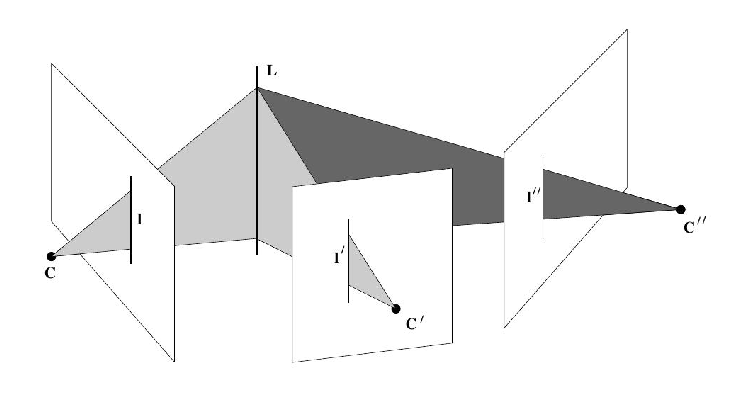
\includegraphics[scale=1]{abord-geo-tri}
\caption{{\it O desenvolvimento algébrico do tensor trifocal realizado a partir das três imagens de uma reta no espaço 3D.}}
\label{fig.abord-geo-tri}
\end{figure}
Considerando $\alpha$, $\beta$ e $k$ escalares, o posto dois de $M$ pode ser interpretado com uma dependência linear entre suas colunas, e como
\begin{equation*}
M=
\begin{bmatrix}
\lightrgb&A^\top\lightrgb'&B^\top\lightrgb''\\
0&{\bf a}^\top_4\lightrgb'&
{\bf b}^\top_4\lightrgb''
\end{bmatrix}
\end{equation*}
podemos definir o sistema
\begin{equation}\label{eq.sistema-tri}
\begin{pmatrix}
\lightrgb\\
0
\end{pmatrix}
=
\alpha
\begin{pmatrix}
A^\top\lightrgb'\\
{\bf a}^\top_4\lightrgb'
\end{pmatrix}
+\beta
\begin{pmatrix}
B^\top\lightrgb''\\
{\bf b}^\top_4\lightrgb''
\end{pmatrix}.
\end{equation}
Pela quarta equação do sistema \ref{eq.sistema-tri} temos
\begin{equation*}
\alpha=k\,{\bf b}^\top_4\lightrgb''\quad\text{e}\quad\beta=-k\,{\bf a}^\top_4\lightrgb'\quad\Rightarrow\quad0=\alpha\,{\bf a}^\top_4\lightrgb'+\beta\,{\bf b}^\top_4\lightrgb''.
\end{equation*}
Substituindo os valores de $\alpha$ e $\beta$ nas três primeiras equações do sistema \ref{eq.sistema-tri} e desconsiderando o fator de escala $k$, temos
\begin{equation*}
\begin{array}{rcl}
\lightrgb&=&\alpha\,A^\top\lightrgb'+\beta\,B^\top\lightrgb''\\
\lightrgb&=&({\bf b}^\top_4\lightrgb'')A^\top\lightrgb'-({\bf a}^\top_4\lightrgb')B^\top\lightrgb''\\
\lightrgb&=&(\lightrgb''^\top{\bf b}_4)A^\top\lightrgb'-(\lightrgb'^\top{\bf a}_4)B^\top\lightrgb''.
\end{array}
\end{equation*}
A $i$-ésima coordenada de $\lightrgb$ pode ser dada por
\begin{equation*}
\begin{array}{rcl}
l_i&=&\lightrgb''^\top({\bf b}_4{\bf a}^\top_i)\lightrgb'-\lightrgb'^\top({\bf a}_4{\bf b}_i^\top)\lightrgb''\\
l_i&=&\lightrgb'^\top({\bf a}_i{\bf b}^\top_4)\lightrgb''-\lightrgb'^\top({\bf a}_4{\bf b}_i^\top)\lightrgb''\\
l_i&=&\lightrgb'^\top({\bf a}_i{\bf b}^\top_4-{\bf a}_4{\bf b}_i^\top)\lightrgb''\\
l_i&=&\lightrgb'^\top \mbox{T}_i\lightrgb'',
\end{array}
\end{equation*}
onde definimos $\mbox{T}_i={\bf a}_i{\bf b}^\top_4-{\bf a}_4{\bf b}_i^\top$. 
O conjunto das três matrizes $\left\{\mbox{T}_1,\mbox{T}_2,\mbox{T}_3\right\}$ é denominado {\it tensor trifocal} e a reta $\lightrgb$ é dada por
\begin{equation}\label{eq.tres-retas}
\lightrgb=
\begin{pmatrix}
\lightrgb'^\top \mbox{T}_1\lightrgb''\\
\lightrgb'^\top \mbox{T}_2\lightrgb''\\
\lightrgb'^\top \mbox{T}_3\lightrgb''
\end{pmatrix}.
\end{equation}

\subsubsection{Homografia induzida por um plano}\label{sec.homo-plano-tri}
Vimos na subseção anterior que podemos determinar o tensor trifocal através da relação entre três retas correspondentes, mas existem mais quatro relações entre retas e pontos  correspondentes envolvendo o tensor trifocal. Para derivarmos essas outras relações e voltarmos ao problema da transferência de pontos, precisamos definir a homografia entre a primeira e terceira imagens induzida por um plano $\bpi'$, retroprojetado por uma reta $\lightrgb'$ na segunda imagem, conforme a figura \ref{fig.transfer-retas}.
\begin{figure}[!htb]
\centering
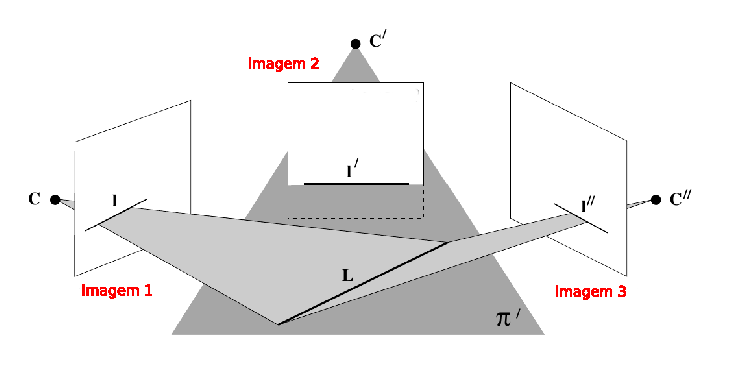
\includegraphics[scale=1]{transfer-retas}
\caption{{\it O plano $\bpi'$ retroprojetado por $\lightrgb'$ induz uma homografia que relaciona $\lightrgb$ com $\lightrgb''$.}}
\label{fig.transfer-retas}
\end{figure}
As homografias entre pontos e retas em dois planos são dadas, respectivamente, por $\x''=H\,\x$ e $\lightrgb''=H^{-\top}\lightrgb$ (subseção \ref{sec.trans-proj-H}). Invertendo $H^{-\top}$ temos que $\lightrgb=H^\top\lightrgb''$. Como temos três retas correspondentes que satizfazem a relação \ref{eq.tres-retas}, podemos comparar essa relação com $\lightrgb=H^\top\lightrgb''$ e deduzir que $H=[\mbox{T}_1^\top\lightrgb',\mbox{T}_2^\top\lightrgb',\mbox{T}_3^\top\lightrgb']$, pois
\begin{equation*}
\lightrgb=
\begin{pmatrix}
\lightrgb'^\top \mbox{T}_1\lightrgb''\\
\lightrgb'^\top \mbox{T}_2\lightrgb''\\
\lightrgb'^\top \mbox{T}_3\lightrgb''
\end{pmatrix}=
\begin{pmatrix}
(\mbox{T}_1^\top\lightrgb')^\top\lightrgb''\\
(\mbox{T}_2^\top\lightrgb')^\top\lightrgb''\\
(\mbox{T}_3^\top\lightrgb')^\top\lightrgb''
\end{pmatrix}=
\begin{pmatrix}
{\bf h}_1^\top\lightrgb''\\
{\bf h}_2^\top\lightrgb''\\
{\bf h}_3^\top\lightrgb''
\end{pmatrix}=
\begin{bmatrix}
{\bf h}_1^\top\\
{\bf h}_2^\top\\
{\bf h}_3^\top
\end{bmatrix}\,\lightrgb''=
H^\top\lightrgb'',
\end{equation*}
onde tomamos ${\bf h}_i=\mbox{T}_i^\top\lightrgb'$.
A homografia deduzida acima (denotada por $H_{13}$) representa a transformação de um ponto da primeira imagem para a terceira através de uma reta na segunda imagem, $\x''=H_{13}\x$. Analogamente, podemos deduzir a homografia da primeira imagem para a segunda através de uma reta na terceira imagem, $\x'=H_{12}\x$.

\subsubsection{Relações de incidência entre pontos e retas}\label{sec.rela-incidi-tri}
Uma das relações de incidência já foi deduzida anteriormente, chamada reta-reta-reta, e agora vamos deduzir mais quatro relações. Supondo ainda $\lightrgb$, $\lightrgb'$ e $\lightrgb''$ três imagens de uma reta ${\bf L}$, sabemos que um ponto $\x$ pertence à uma reta $\lightrgb$ na câmera 1 se $\x^\top\lightrgb=0$, onde a multiplicação matricial pode ser escrita sob a notação de somatório como $\sum_{i=1}^{3}x^il_i=0$. O índice contravariante em $x$ é uma conveção para facilitar o algebrismo na notação padrão de tensor trifocal. Essa convensão se deve ao fato de que o tensor trifocal possui três índices e não apenas dois como ocorre com as matrizes. A equação \ref{eq.tres-retas} pode ser dada como $\lightrgb'^\top \mbox{T}_i\lightrgb''
=l_i$ para $i=1,2,3$, e usando o somatório temos que
\begin{equation*}
\begin{array}{rcl}
\lightrgb'^\top \mbox{T}_i\lightrgb''
&=&l_i\\
\sum_{i=1}^3 x^i(\lightrgb'^\top \mbox{T}_i\lightrgb'')&=&\sum_{i=1}^3 x^il_i\\
\lightrgb'^\top(\sum_{i=1}^3 x^i\mbox{T}_i)\lightrgb''&=&0.
\end{array}
\end{equation*}
Desta forma, temos a segunda relação de incidência chamada ponto-reta-reta, para um ponto $\x$ na primeira imagem e as retas $\lightrgb'$ e $\lightrgb''$ na segunda e terceira imagens respectivamente. 

Pela subseção \ref{sec.proj.retas} sabemos da existência de um ponto $\X\in{\bf L}$ que projeta $\x\in\lightrgb$ na primeira imagem e projeta a outros dois pontos $\x'\in\lightrgb'$ e $\x''\in\lightrgb''$, ou seja, temos a correspondência $\x\leftrightarrow\x'\leftrightarrow\x''$. Assim, podemos deduzir as relações para 
pontos na segunda e terceira imagens utilizando a homografia induzida por plano, e vamos tratar da terceira relação de incidência, o caso ponto-reta-ponto. Usando o resultado da subseção \ref{sec.homo-plano-tri} temos que 
\begin{equation*}
\begin{array}{rcl}
\x''&=&H_{13}\x\\
&=&[\mbox{T}_1^\top\lightrgb',\mbox{T}_2^\top\lightrgb',\mbox{T}_3^\top\lightrgb']\x\\
&=&
\begin{pmatrix}
x_1\mbox{T}_1^\top\lightrgb'+x_2\mbox{T}_2^\top\lightrgb'+x_3\mbox{T}_3^\top\lightrgb'
\end{pmatrix}\\
&=&(\sum_{i=1}^3 x^i\mbox{T}_i^\top)\,\lightrgb'
\end{array}
\end{equation*}
Como estamos expressando os vetores em coordenadas homogêneas, essas equações são invariantes para a aplicação de um fator de escala. De qualquer maneira, podemos eliminar o problema das diferenças de escala aplicando a transposição seguida do produto vetorial à direita em ambos os lados da equação
\begin{equation}\label{eq.ponto-reta-ponto}
\begin{array}{rcl}
\x''&=&(\sum_{i=1}^3 x^i\mbox{T}_i^\top)\,\lightrgb'\\
\x''^\top&=&\lightrgb'^\top(\sum_{i=1}^3 x^i\mbox{T}_i)\\
\x''^\top[\x'']_\times&=&\lightrgb'^\top(\sum_{i=1}^3 x^i\mbox{T}_i)[\x'']_\times\\
{\bf 0}^\top&=&\lightrgb'^\top(\sum_{i=1}^3 x^i\mbox{T}_i)[\x'']_\times.
\end{array}
\end{equation}
O quarto caso, ponto-ponto-reta, é análogo ao apresentado aqui substituindo $\x''$ por $\x'$, e usando a homografia induzida pelo plano retroprojetado por $\lightrgb''$, $\x'=H_{12}\x$.

Por último, temos a relação de incidência para três pontos. 
Observe que a reta $\lightrgb'$ na relação \ref{eq.ponto-reta-ponto} pode ser definida como $\lightrgb'=\x'\times \y'=[\x']_\times \y'$, já que $\x'\in\lightrgb'$ e $\y'$ é um ponto qualquer no plano da segunda imagem. Substituindo $\lightrgb'$, a relação \ref{eq.ponto-reta-ponto} se torna 
\begin{equation*}
\y'^\top[\x']_\times(\sum_{i=1}^3 x^i\mbox{T}_i)[\x'']_\times={\bf 0}^\top,
\end{equation*}
mas observa-se que tal relação é válida para qualquer reta $\lightrgb'$ que seja imagem de ${\bf L}$, e portanto não depende da escolha do ponto $\y'$ que pode ser descartado. A relação ponto-ponto-ponto é
\begin{equation*}
[\x']_\times(\sum_{i=1}^3 x^i\mbox{T}_i)[\x'']_\times=0_{3\times3}.
\end{equation*}
Cabe resaltar que apenas satisfazer qualquer das relações de incidência não garante a incidência no espaço 3D, ou seja, o tensor trifocal obtido pode não ter consistência com a geometria trifocal de abordagem do problema.

\subsubsection{Relação de incidência para retas epipolares}\label{sec.rela-reta-epipolar-tri}
Suponha que os planos retroprojetados por $\lightrgb$ e $\lightrgb'$ sejam coincidentes e que o ponto 3D $\X$ pertença a esse plano denotado por $\bpi'$, de acordo com a figura \ref{fig.plano-epipolar-tri}. Neste caso, $\bpi'$ é o plano epipolar para as câmeras 1 e 2, e a reta retroprojetada por $\x$, imagem de $\X\in{\bf L}$, está inteiramente contida em $\bpi'$. Como dois planos não coincidentes sempre definem uma reta, o plano retroprojetado por $\lightrgb''$ intercepta o plano $\bpi'$ em ${\bf L}$. Já que a reta retroprojetada por $\x$ está inteiramente contida em $\bpi'$, essa reta deverá interceptar a reta ${\bf L}$ no ponto $\X$. Desta forma, pela subseção \ref{sec.rela-incidi-tri}, temos a correspondência $\x\leftrightarrow\lightrgb'\leftrightarrow\lightrgb''$ que satisfaz a relação
\begin{equation*}
\lightrgb'^\top(\sum_{i=1}^3 x^i\mbox{T}_i)\lightrgb''=0.
\end{equation*}
Observe que, como dois planos sempre definem uma reta, a incidência não depende da escolha do plano retroprojetado pela câmera 3, ou seja, essa incidência vai ocorrer qualquer que seja a reta $\lightrgb''$. Consequentemente, a relação anterior não depende de $\lightrgb''$, e pode ser reduzida a 
\begin{equation}\label{eq.rela-incide-epipolar}
\lightrgb'^\top(\sum_{i=1}^3 x^i\mbox{T}_i)={\bf 0}^\top\quad\text{ou}\quad(\sum_{i=1}^3 x^i\mbox{T}_i)\lightrgb''={\bf 0}.
\end{equation}
A argumentação é análoga considerando o plano epipolar definido pelas retas $\lightrgb$ e $\lightrgb''$, e neste caso a relação será independente da posição da reta $\lightrgb'$. 
\begin{figure}[!htb]
\centering
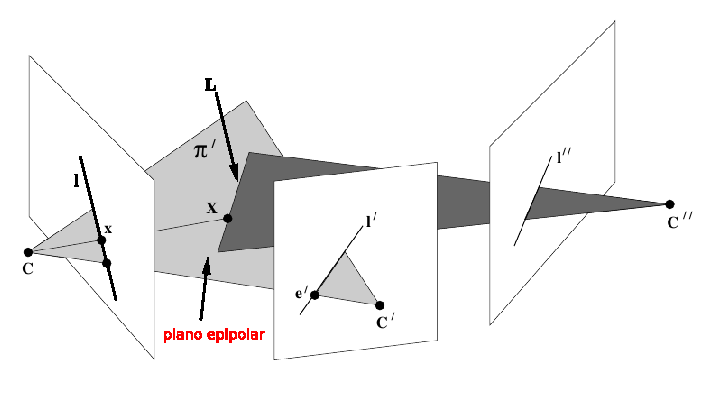
\includegraphics[scale=1]{plano-epipolar-tri}
\caption{{\it Quando ${\bf L}$ pertence a um plano epipolar definido para duas imagens, a relação de incidência $\x\leftrightarrow\lightrgb'\leftrightarrow\lightrgb''$ não depende da reta numa terceira imagem.}}
\label{fig.plano-epipolar-tri}
\end{figure}

Pelas relações em \ref{eq.rela-incide-epipolar} notamos que é possível calcular as retas epipolares como o espaço nulo da matriz $\sum_{i=1}^3 x^i \mbox{T}_i$. Variando o ponto $\x$ é possível obter várias retas epipolares, e todas passam pelo mesmo epipolo. Assim, podemos calcular os epipolos $\e'$ e $\e''$ como interseção dessas retas. Tal resultado será importante na abordagem sobre reconstrução 3D por ocasião da extração das matrizes das câmeras a partir do tensor trifocal.

\subsection{Transferências usando o tensor trifocal}

\subsubsection{Transferência de pontos}
A primeira vantagem no uso do tensor trifocal é que, dos casos de degeneração apresentados na subseção \ref{sec.trans-epipolar}, apenas um deles não pode ser resolvido pelo uso do tensor, como veremos a seguir. 

Considere novamente que se deseja, dada a correspondência entre pontos nas duas primeiras imagens $\x\leftrightarrow\x'$, determinar as coordenadas do ponto correspondente na terceira imagem, $\x''$. Escolhendo uma reta $\lightrgb'$ passando por $\x'$ na segunda imagem e de posse do tensor trifocal, podemos utilizar a relação de incidência 
\begin{equation}\label{eq.ponto-reta-ponto-isolada}
\x''=(\sum_{i=1}^3 x^i\mbox{T}_i^\top)\,\lightrgb'
\end{equation} 
deduzida na subseção \ref{sec.rela-incidi-tri}
para computar diretamente $\x''$. Devemos apenas ter um pouco de cuidado na escoha da reta $\lightrgb'$, pois no caso de ser a reta epipolar correspondente a $\x$ temos, pela subseção \ref{sec.rela-reta-epipolar-tri}, que $(\sum_{i=1}^3 x^i\mbox{T}_i^\top)\,\lightrgb'={\bf 0}$, e o ponto $\x''$ não pode ser determinado. Uma das formas de resolver o problema seria escolher duas ou três retas passando por $\x'$, computar o ponto $\x''$ e escolher aquele que apresenta a maior norma. Outra opção, caso tenha extraído a matriz fundamental $F_{21}$ para as câmeras 1 e 2, é calcular a reta epipolar $\lightrgb'_{\e}=F_{21}\x$ e escolher $\lightrgb'$ que seja perpendicular a $\lightrgb'_{\e}$, ou seja, $\lightrgb'^\top\lightrgb'_{\e}=0$. 

Considere, pela figura \ref{fig.trifocal-frente}, o caso onde o ponto $\X$ está alojado na reta base definida por $\C$ e $\C'$. Nessa posição, a imagem de $\X$ na câmera 2 é o epipolo $\e_{21}=\x'$. Para escolha de qualquer reta que passe por $\x'$ para aplicarmos a relação \ref{eq.ponto-reta-ponto-isolada}, estaremos escolhendo uma reta epipolar, e como vimos anteriormente, não poderemos definir a posição do ponto $\x''$. Tal reta base é o único lugar que $\X$ pode se alojar no plano trifocal que não permite que o ponto $\x''$ seja calculado usando o tensor trifocal, em contraste com a transferência epipolar que se degenera para qualquer $\X$ no plano trifocal. Observe pela figura \ref{fig.X-plano-trifocal} que, desde que a reta ${\bf L}$ não pertença ao plano trifocal, não há motivos para a degeneração da transferência usando o tensor trifocal à medida que variamos a posição de $\X$ em ${\bf L}$. 
\begin{figure}[!htb]
\centering
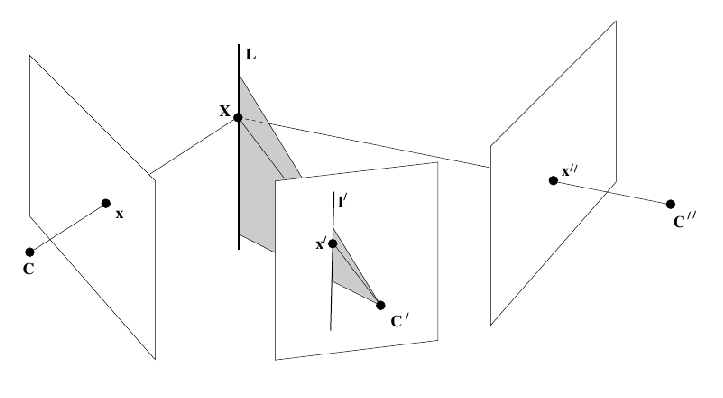
\includegraphics[scale=1]{X-plano-trifocal}
\caption{{\it Desde de que ${\bf L}$ não pertença ao plano trifocal, não há motivos para degenerações à medida que variamos $\X$ em ${\bf L}$.}}
\label{fig.X-plano-trifocal}
\end{figure}
No caso onde os centros das câmeras estão alinhados, não poderemos determinar a posição de $\x''$ caso $\X$ esteja em quaisquer das três retas base, já que assim essas três retas são uma reta só. Lembramos que a transferência epipolar falha para centros de projeção alinhados qualquer que seja a posição de $\X$.  

\subsubsection{Transferência de retas}
Podemos realizar a transferência de retas utilizando a relação
\begin{equation*}
\lightrgb=
\begin{pmatrix}
\lightrgb'^\top \mbox{T}_1\lightrgb''\\
\lightrgb'^\top \mbox{T}_2\lightrgb''\\
\lightrgb'^\top \mbox{T}_3\lightrgb''
\end{pmatrix},
\end{equation*}
que dá uma maneira explícita de calcularmos a reta na primeira imagem dadas as retas nas câmeras 2 e 3. Mas podemos calcular retas em quaisquer das três imagens dadas as outras duas, aplicando o produto vetorial por $\lightrgb$ em ambos os lados da equação
\begin{equation*}
\begin{array}{rcl}
\lightrgb\times\lightrgb&=&\lightrgb\times
\begin{pmatrix}
\lightrgb'^\top \mbox{T}_1\lightrgb''\\
\lightrgb'^\top \mbox{T}_2\lightrgb''\\
\lightrgb'^\top \mbox{T}_3\lightrgb''
\end{pmatrix}\\
{\bf 0}&=&\lightrgb\times
\begin{pmatrix}
\lightrgb'^\top \mbox{T}_1\lightrgb''\\
\lightrgb'^\top \mbox{T}_2\lightrgb''\\
\lightrgb'^\top \mbox{T}_3\lightrgb''
\end{pmatrix}.\\
\end{array}
\end{equation*}
O sistema fornece três equações, sendo duas independentes, para determinar os dois graus de liberdade da reta procurada. Outra vantagem no uso de tensor trifocal é que retas explícitas não podem ser determinadas usando apenas matrizes fundamentais.

Repare, pela figura \ref{fig.plano-epipolar-tri}, que se as retas $\lightrgb$ e $\lightrgb'$ retroprojetam o mesmo plano, então não teremos uma única reta definida em 3D que possa ser projetada na terceira imagem, e essas duas retas são retas epipolares correspondentes. Similarmente, não podemos determinar a reta na segunda imagem caso as retas na primeira e terceira imagens sejam retas epipolares correspondentes. Em posições gerais, não há motivo para a geometria epipolar entre as câmeras 1 e 2, e câmeras 1 e 3 serem iguais, ou seja, os dois tipos de transferência não se degeneram simultaneamente com frequência. No entanto, assim como pontos na tranferência epipolar, não é possível aplicar a transferência através do tensor trifocal se a reta 3D estiver contida no plano trifocal. 

\subsection{Reconstrução das câmeras a partir do tensor trifocal}
Assim como foi mostrado no caso bifocal, mostraremos agora como extrair as matrizes fundamentais e as matrizes das câmeras a partir do tensor trifocal.

\subsubsection{Extração da matriz fundamental}\label{sec.extracao-F-tri}
Considerando um ponto $\x$ na primeira imagem, como vimos na subseção \ref{sec.homo-plano-tri}, temos uma homografia que relaciona a primeira com a terceira imagem através de um plano retroprojetado por uma reta $\lightrgb'$ na segunda imagem, conforme a figura \ref{fig.transfer-retas}. Com isso, podemos definir a reta epipolar $\lightrgb''$ na terceira imagem relativa ao ponto $\x$ na primeira imagem. O ponto $\x''$ na terceira imagem é dado por
\begin{equation*}
\x''=H_{13}\x\quad\text{ou}\quad\x''=[\mbox{T}_1^\top\lightrgb',\mbox{T}_2^\top\lightrgb',\mbox{T}_3^\top\lightrgb']\,\x,
\end{equation*}  
e a reta epipolar na terceira imagem pode ser calculada como $\lightrgb''=\e''\times\x''$. Substituindo a expressão para $\x''$ temos
\begin{equation*}
\begin{array}{rcl}
\lightrgb''&=&\e''\times\x''\\
\lightrgb''&=&[\e'']_\times[\mbox{T}_1^\top\lightrgb',\mbox{T}_2^\top\lightrgb',\mbox{T}_3^\top\lightrgb']\,\x\\
\lightrgb''&=&F_{31}\,\x,
\end{array}
\end{equation*}
onde a matriz fundamental pode ser obtida por $F_{31}=[\e'']_\times[\mbox{T}_1^\top\lightrgb',\mbox{T}_2^\top\lightrgb',\mbox{T}_3^\top\lightrgb']$.

Algebricamente esta expressão se mantém para qualquer reta $\lightrgb'$, mas devemos escolher uma reta para evitar a condição de degeneração onde $\mbox{T}^\top_i\lightrgb'={\bf 0}$. Uma boa escolha é tomar $\lightrgb'=\e'$ pois $\e'$ é perpendicular ao espaço nulo à direita de cada $\mbox{T}^\top_i$. Assim , a matriz fundamental é obtida simplesmente por
\begin{equation*}
F_{31}=[\e'']_\times[\mbox{T}_1^\top\e',\mbox{T}_2^\top\e',\mbox{T}_3^\top\e'].
\end{equation*} 
Uma análise similar permite verificar que podemos obter uma relação que envolve a segunda e primeira imagens,
\begin{equation*}
F_{21}=[\e']_\times[\mbox{T}_1\e'',	\mbox{T}_2\e'',\mbox{T}_3\e''].
\end{equation*}

\subsubsection{Extraindo as matrizes das câmeras}

Da mesma forma que acontece no caso bifocal, por conta da ambiguidade projetiva, podemos determinar as matrizes das câmeras tomando a câmera 1 como $P=[I|{\bf 0}]$ aplicando uma transformação projetiva. Seguindo a subseção \ref{sec.cameras-canonicas}, dadas duas câmeras $P=[I|{\bf 0}]$ e $P'=[M|{\bf m}]$, a matriz fundamental é extraída como $F=[{\bf m}]_\times M$. Usando a matriz fundamental $F_{21}=[\e']_\times[\mbox{T}_1\e'',	\mbox{T}_2\e'',\mbox{T}_3\e'']$ extraída do tensor trifocal na subseção \ref{sec.extracao-F-tri}, temos que o par de câmeras, dado o tensor trifocal é
\begin{equation}\label{eq.deducao-simples-P-tri}
P=[I|{\bf 0}]\quad\text{e}\quad P'=[[\mbox{T}_1\e'',\mbox{T}_2\e'',\mbox{T}_3\e'']|\e'].
\end{equation}

Poderíamos pensar que as câmeras 1 e 3 poderiam ser obtidas usando a matriz fundamental $F_{31}=[\e'']_\times[\mbox{T}_1^\top\e',\mbox{T}_2^\top\e',\mbox{T}_3^\top\e']$, e daí a câmera 3 seria $P''=[[\mbox{T}_1^\top\e',\mbox{T}_2^\top\e',\mbox{T}_3^\top\e']|\e'']$, mas está {\it incorreto}. A câmera 3 não pode ser escolhida independentemente das características projetivas das câmeras 1 e 2. Pois, observe que podemos reconstruir o ponto 3D $\X$ a partir das câmeras 1 e 2, e usá-lo para determinar a câmera 3 usando as correspondências $\X\leftrightarrow\x''$, conforme o artigo na seção \ref{sec.astrom}. Assim, $P''$ depende das características projetivas do par $(P,P')$. 

De acordo com a subseção \ref{sec.ambi-cameras-dada-F} e usando a dedução dada pela equação \ref{eq.deducao-simples-P-tri}, uma forma mais geral de se obter $P$ e $P'$ é dada por
\begin{equation}\label{eq.familia-cameras}
P=[I|{\bf 0}]\quad\text{e}\quad P'=[[\mbox{T}_1\e'',\mbox{T}_2\e'',\mbox{T}_3\e'']+\e'^\top{\bf v} |\lambda\,\e'],
\end{equation}    
para algum vetor ${\bf v}$ e um escalar $\lambda$. E para determinarmos $P''$ devemos obter um trio de câmeras dessa família que seja compatível com a dedução do tensor trifocal dada na subseção \ref{sec.tensor-tri-rela-inci},
\begin{equation}\label{eq.tensor-tri}
\mbox{T}_i={\bf a}_i{\bf b}_4^\top-{\bf a}_4{\bf b}_i^\top,
\end{equation}
onde ${\bf a}_i$ são a colunas de $P'$ e ${\bf b}_i$ são as colunas de $P''$.
Por conta da ambiguidade projetiva, dentre essa família de câmeras em \ref{eq.familia-cameras}, podemos escolher $P'=[[\mbox{T}_1\e'',\mbox{T}_2\e'',\mbox{T}_3\e'']|\e']$ para desta forma termos ${\bf a}_i=\mbox{T}_i\e''$ para $i=$1,2 e 3. Notando que ${\bf a}_4=\e'$ e ${\bf b}_4=\e''$, podemos substituir as três últimas relações na equação \ref{eq.tensor-tri} e obter
\begin{equation*}
\mbox{T}_i=\mbox{T}_i\e''\e''^\top-\e'{\bf b}_i^\top,
\end{equation*}
onde, isolando ${\bf b}_i^\top$ temos 
\begin{equation}\label{eq.deri-parcial-P''}
\e'{\bf b}_i^\top=\mbox{T}_i (\e''\e''^\top-I)
\end{equation}
Como o fator de escala é irrelevante, podemos escolher $\e'$ de forma que $\e'^\top\e'=1$, multiplicar $\e'^\top$ pela esquerda na relação \ref{eq.deri-parcial-P''} e aplicar a transposta para chegarmos a
\begin{equation*}
{\bf b}_i=(\e''\e''^\top -I)\mbox{T}_i^\top\e'.
\end{equation*}
Agora podemos definir a câmera 3 considerando as características projetivas das câmeras 1 e 2,
\begin{equation*}
P''=[(\e''\e''^\top -I)[\mbox{T}_1^\top\e',\mbox{T}_2^\top\e',\mbox{T}_3^\top\e']|\e''],
\end{equation*}
e assim verificarmos que o tensor trifocal determina completamente as matrizes das câmeras a menos de uma ambiguidade projetiva.

